\setchapterpreamble[u]{\margintoc}
\chapter{Trustworthiness Through Experiments: Copyright Traps}



\begin{kaobox}[frametitle=Paper Abstract]

Questions of fair use of copyright-protected content to train Large Language Models (LLMs) are being actively debated. Document-level inference has been proposed as a new task: inferring from black-box access to the trained model whether a piece of content has been seen during training. SOTA methods however rely on naturally occurring memorization of (part of) the content. While very effective against models that memorize significantly, we hypothesize--and later confirm--that they will not work against models that do not naturally memorize, e.g. medium-size 1B models. We here propose to use copyright traps, the inclusion of fictitious entries in original content, to detect the use of copyrighted materials in LLMs with a focus on models where memorization does not naturally occur. We carefully design a randomized controlled experimental setup, inserting traps into original content (books) and train a 1.3B LLM from scratch. We first validate that the use of content in our target model would be undetectable using existing methods. We then show, contrary to intuition, that even medium-length trap sentences repeated a significant number of times (100) are not detectable using existing methods. However, we show that longer sequences repeated a large number of times can be reliably detected (AUC=0.75) and used as copyright traps. 
Beyond copyright applications, our findings contribute to the study of LLM memorization: the randomized controlled setup enables us to draw causal relationships between memorization and certain sequence properties such as repetition in model training data and perplexity.

\end{kaobox}

\section{Introduction}





With the growing adoption of ever-improving Large Language Models (LLMs), concerns are being raised when it comes to the use of copyright protected content for training. 
Numerous content creators have indeed filed lawsuits against technology companies, claiming copyright infringement for utilizing books\sidecite{authorsguild, silvermanmeta}, songs\sidecite{anthropic} or news articles\sidecite{nytimes} for LLM development. While it is still unclear whether copyright or \emph{fair use} applies in this context\sidecite{samuelson2023generative}, model developers continue releasing new LLMs but are increasingly reluctant to disclose details on the training dataset\sidecite{openai_gpt-4_2023, touvron_llama_2023, jiang2024mixtral} - partially due to these lawsuits. 

Methods have recently been developed to detect whether a specific piece of content has been seen by an LLM during training: document-level membership inference. Both\sidecite{meeus2023did} and\sidecite{shi2023detecting} show their methods to be fairly successful against very large LLMs (up to 66B parameters), with a ROC AUC of 0.86 for OpenLLaMA\sidecite{openlm2023openllama} and 0.88 for GPT-3\sidecite{brown_language_2020}.

\begin{figure}[t]
\centering
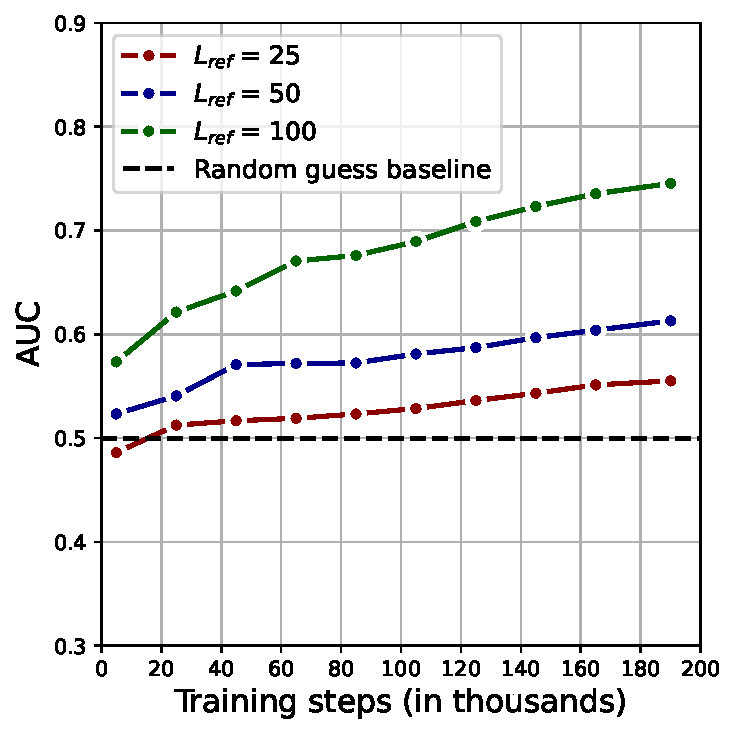
\includegraphics[width=0.6\linewidth] {images/copyright_traps_figures/MIAOverTraining.pdf} 
    \caption[Memorization throughout training]{\textbf{Memorization throughout training.} The \textit{Ratio} MIA performance (AUC) for synthetically generated trap sequences (of varying sequence length), repeated 1,000 times in a book, evaluated on intermediate checkpoints of the target LLM.}
    %The full training corresponds to 2 epochs.} 
\label{fig:across_training}
\end{figure}

Historically, original content creators have implemented so-called \emph{copyright traps} to detect copyright infringement of their work. Examples of such traps range from a fictitious street name or town on a map to the inclusion of fabricated names in a dictionary\sidecite{Alford_2005a}. In this case, the direct inclusion of these entities in other work would render a breach of copyright self-evident, while it becomes less trivial when data is aggregated, e.g. when used in machine learning models. 

We here investigate, for the first time, the use of copyright traps for document-level membership inference against LLMs. We propose the injection of purposefully designed text (\emph{trap sequences}) into a piece of content, to either further improve the performance of document-level membership inference or enable it in the first place for models less prone to memorization. 

We here focus on the latter, as recently proposed methods are already successful for larger models\sidecite{meeus2023did, shi2023detecting}, and as there is a growing trend towards smaller language models\sidecite{zhang2024tinyllama, Javaheripi_2023}. 

Specifically, we inject our traps into the training set of CroissantLLM\sidecite{faysse_croissantllm_2024}, a 1.3B parameter LLM, trained from scratch on 3 trillion tokens by the team we partnered with. Being (fairly) small and trained on significantly more data than considered in prior work on LLM memorization\sidecite{carlini2022quantifying}, we hypothesized that the model would not naturally memorize sufficiently for a document-level membership inference to succeed. Applying the two state-of-the-art methods\sidecite{meeus2023did, shi2023detecting}, we find them to perform barely better than a random guess baseline, confirming our hypothesis and rendering these methods uninformative for authors. 

We hence investigate the use of document-specific copyright traps to enable membership inference. We apply Membership Inference Attacks (MIAs) from the literature\sidecite{yeom2018privacy, carlini2021extracting, shi2023detecting} to infer whether a given trap sequence, and thus document, has been seen by a model or not.

First, we consider synthetically generated trap sequences and study the impact of number of repetitions, sequence length, and perplexity  on the post training detectability of the trap. Contrary to popular beliefs, notably from the training data extraction literature\sidecite{carlini2021extracting, nasr2023scalable}, we show that short and medium-length synthetic sequences repeated a significant number of times (100) do not help the membership inference, independently of the detection method used. We further confirm this also holds for artificially duplicated existing sentences. 

We, however, do find that the MIA AUC increases with sequence length and number of repetitions and that sequences of 100 tokens repeated 1,000 times are detectable with an AUC of 0.748. This provides the first evidence that copyright traps can be inserted in real-world LLMs to detect the use of training content otherwise undetectable.
% whose use of certain content would otherwise not be detectable. 

%In a post-hoc analysis, we demonstrate the impact of the number of times a sequence has been seen by the model on detectability. More specifically, we track the memorization during the training process, by computing the MIA AUC for our trap sequences across intermediate model checkpoints. We find that the AUC -and thus LLM memorization- increases smoothly and monotonically with the training steps, with no sign of reaching a plateau. 

We also show that sequences with high-perplexity (according to a reference model) are more likely to be detectable. The general intuition is that 'outliers' might more easily be memorized and be more vulnerable against MIAs\sidecite{feldman2020does}. We are the first to test this out for LLMs in a clean setup, and show that when memorization happens (for long sequences repeated 1,000 times), the MIA AUC improves from approximately 0.65 for low perplexity to 0.8 for high perplexity. We also show the relationship between perplexity and detectability to be a potential confounding factor in prior post-hoc studies of LLM memorization, by studying the perplexity of duplicate sequences in the large text dataset The Pile\sidecite{pile}.

Our results provide the first evidence that target-model independent copyright traps can be added to content to enable document-level membership inference, even in LLMs that would not 'naturally' memorize sufficiently to infer membership. 

While injecting traps might be not be equally trivial across document types while maintaining readability, they can be embedded across a large corpus (e.g. news articles). They can also be hidden online and not trivial to remove, especially given automated scraping and the costs associated with fine-grained deduplication for LLM training data. 


\section{Conclusion}

With the copyright concerns regarding LLM training being raised, LLM developers are reluctant to disclose details on their training data. Prior work has explored the question of document-level membership inference to detect whether a piece of content has been used to train a LLM. We first show that memorization highly depends on the training setup, as existing document-level membership inference methods fail for our 1.3B LLM. We thus propose the use of copyright traps for LLMs - purposefully designed text sequences injected into a document, intended to maximize detectability in LLM training data. 

We train a real-world, 1.3B LLM from scratch on 3 trillion tokens, containing a small set of injected trap sequences, enabling us to study their effectiveness. We find that inducing reliable memorization in a LLM is a non-trivial task. For models showing relatively low level of memorization, such as the one we train here, injecting short-to-medium sentences ($\leq $ 50 tokens) up to a 100 times does not improve document detectability. When using longer sequences, however, and up to a $1,000$ repetitions, we do see a significant effect - showing how copyright traps can enable detactability even for LLMs less prone to memorize. We further find that memorization increases with sequence perplexity, and that leveraging document-level information such as context could boost detectability. While effective, the proposed mechanism could be disruptive to the document's content and readability. Future research is thus needed, specifically in designing trap sequences maximizing detectability. We are hence committed to releasing our model and the data to further the research in the field.
